\chapter{Physical Background }
\label{This chapter bears the basis of fundamental physics in semiconductors and
quantum structures that were implemented to understand the results in this work..}
\vfill
\minitoc
\newpage

\lettrine[lines=3, lraise=.1, nindent=0mm, slope=0mm]{\textbf{Q}}{uantum mechanics}  is basically electron behavior that exhibits many phenomena non explained by classical regime. Quantum structures (QS) are artificially systems conformed by semiconductors where electrons exhibit their quantum nature, this is a great platform to study and create quantum devices. Nowadays, the progress in creation of QS consist in precisely deposition of thin films, in which electrons show fundamentally new electrical and optical properties\cite{sundram1991structures}. Most of these properties consist in quantum behavior  as the energy confinement, which is the principal interest to study the electron and their consequent interactions which generates analogous  hydrogen atom in semiconductors. Therefore, the interest to studying QS was increasing for many years ago and nowadays, those continue considering an excellent research area.  

In this chapter, it presents the fundamental concepts to describe the physical  phenomena resultant in this work, without intention to replicate concepts and models already explained in publications with major impact. Therefore, the purpose is to present an own interpretation to highlight the great obtained results.

\section{Semiconductor Bandstructure}
\label{sec:chapter-1-semiconductor}
\vspace{-10mm}
To starting with physical background to understand the QS, it has to start with understand the  band structure of semiconductors. The band structure describes the electron behavior in a solid, therefore, we will need to invoke the \sch equation to describe it behavior. But, due inside a solid around $10^{23}$ valence electrons contribute to the bonding in each cubic centimeter, this results in a many-body complex problem\cite{piprek2017handbook}, then the general hamiltonian for a solid has the form\cite{alloul2010introduction,cardona2005fundamentals}: 

\begin{equation}
\begin{split}
	H  =  &\dfrac{1}{2M}\sum\limits_{i=1}^{N_{n}} \bff{P}_{j}^{2} + \dfrac{1}{2m_{0}} \sum\limits_{j=1}^{N_{e}} \bff{p}_{j}^{2} + \dfrac{Z^{2}}{2} \sum\limits_{i,j=1,i\neq j}^{N_{n}} V_{c}\left(\bff{R}_{i}-\bff{R}_{j}\right)-Z\sum\limits_{i=1}^{N_{n}}\sum\limits_{j=1}^{N_{e}}V_{c}\left(\bff{r}_{j}-\bff{R}_{i}\right) \\
	   & + \dfrac{1}{2} \sum\limits_{i,j=1,i\neq j}^{N_{e}} V_{c} \left(\bff{r}_{i}-\bff{r}_{j}\right),
\end{split}
\label{eq:chapter-1-solid-hamiltonian}
\end{equation}

Where  $N_{n}$ is the number of atomic nuclei, $N_{e}$ is the number of electrons with mass $m_{0}$, asumming that the nuclei are the same mass it's consider  $M$ and charge $Z_{e}$. As is obviously, this Hamiltonian is so complicated, the sum of five terms which consists in : kinetic enrgies to electrons and nuclei, the nucleus-nucleus, nucleus-electron and electron-electron Coulomb interactions, also $\bff{R}_{i}$ are the positions of the nuclei and $\bff{r}_{j}$ are the position of the electrons, the operators $\bff{P}$ and $\bff{p}$ are momentum operators to nuclei and electrons respectively.  Finally, the consider of  Coulomb potential $V_{c}$\cite{alloul2010introduction}.  


Fortunately, the QS are formed by crystalline materials, the Bloch theorem provide the most important tool to develop required equations. The Bloch theorem establish a periodic potential $U(\rv)$ for electrons, this due the material is periodic (definition of crystal structure) and the \sch equation it can describe in terms of single electron  as:  


\begin{equation}
	\left[-\dfrac{\hbar^2}{2m_{0}}\nabla^2 + U(\rv)\right]\psi (r)=\senergy\psi(\rv)
	\label{eq:chapter-1-first-sch}
\end{equation}

The principal reason that the periodic potential in a crystal structure is highly important is their translational invariance concept and the consequent symmetry operations that are possible in a crystalline solid. The symmetry concept, as a  tool to understand solids, is discussed with major detail in the next chapter. In according to Bloch's theorem we can associate a wave vector $\boldsymbol{k}$ with each energy state, $E_{n}(\boldsymbol{k})$. Thus, it is useful to display the energies $E_{n}(\bf{k})$ as a function of the wave vector $\boldsymbol{k}$. This result also knowing as dispersion relation, but in general terms is the electron band structure of the given solid\cite{piprek2017handbook}.   

Even if, the calculation of electron band structure in solids are very complex by the distance between atoms that composes it's, and the Bloch's theorem provide the most important tool to reduce the problem to crystalline structures, exists several methods to  calculate the realistic bandstructure for semiconductors that are categorized in two groups: Atomistic methods\footnote{In this category can include the ab initio methods, these are the most complex methods due to propose  solutions of the many-body problem} (Tight-binding, orthogonalized plane wave methods) and Perturbative methods ($\boldsymbol{k}\bigcdot \boldsymbol{p}$)\footnote{In fact, both TB and $\boldsymbol{k}\bigcdot \boldsymbol{p}$ also consider in same kind, because both are \emph{semi-empirical} methods due to they consider experimental parameters.}. 
These two main categories with theirs respective methods have special characteristics which becomes in the reasons to choose them. The reasons have to do with to the described bandstructure, this mean, in case of Atomistic methods the entire bands  (valence and conduction) can describe, but in case of perturbative methods are reserve to near bandedge bandstructures. So, each of these methods can be chosen and enhanced as the system to study requires. 
We won't enter  in discussion about of which of these methods are the best, the reasons are simple, each method is powerful, and we must be remembered that the complexity of solutions requires that these are solved by numerical techniques therefore this convert it to good approximations. 
Then, basically the electron behavior inside a semiconductor consist in solutions of the appropriate Schrödinger equation\cite{boer2018semiconductor}.  
\subsection{Valence and Conduction Bands}
\label{subsec:chapter-1-valence-and-conduction-bands}
\vspace{-10mm}
The most important characteristic of semiconductors even we can call as the fingerprint of these, is their bands structure, this characteristic sort out the solids as insulators, metals, and semiconductors. 
These are the reason of many mechanisms and phenomena by which study this structures. In general,  the bands of semiconductors composed by valence and conduction bands separated by a  region known as bandgap. 
The bandgap, which is proportional to separation energy of valence and conduction bands also is called as forbidden region, this is because doesn't exist electron states, therefore this gap energy determine the electron conduction in a semiconductor and the difference they have with the insulators and metals as shows \Cref{fig:subsubsection-1.1.1-solid-types}.  

\begin{figure}[h!]
	\centering
	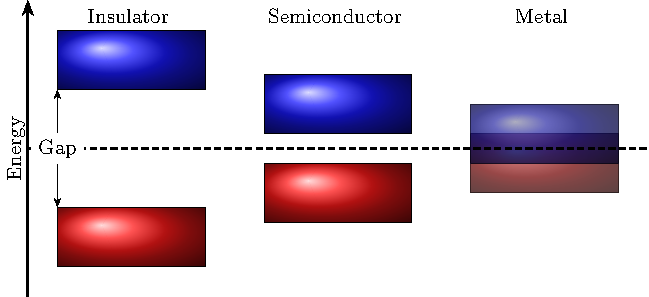
\includegraphics[width=\linewidth]{../figures/chapter-1/solid-sort/build/solid-sort}
	\caption{Band energy diagram for insulators (left), semiconductors(center) and metals (right). The principal difference is the gap energy, for insulators this is longer than semiconductors, although in semiconductors gap energy depends on materials, finally in metals doesn't exist gap energy instead exist an overlap bands characterize these. Dashed line determine Fermi's level.  }
	\label{fig:subsubsection-1.1.1-solid-types}
\end{figure}

So, the bandgap determines many characterizes and functionalities in semiconductors. The bandgap energy classifies semiconductors in direct and indirect semiconductors, but doesn't only depend on this energy, in reality the band structure is the liable for this. As before mentioned, it is so difficult to describe electrons behaviors over the solids due to the many body interactions that exists in its, and therefore the Scr\"odinger equation that's describe electrons behaviors is complicatedly to solve.  Fortunately, the semiconductor structures have a one of the most important characterize  and his has to do with their atomic structure,  that's periodically arrangement of atoms.
This periodicity is the key to propose solutions and describe the semiconductor band structure. 
Starting with describe bulk semiconductors, for example GaAs which consists in with the family III-V cube semiconductor so that their lattice structure consist in a two sublattices correspond to each atom which it conform as shows in \Cref{fig:subsubsection-1.1.1-bulk-1}. For this case, when the atoms in two sublattice are diferent, the crystal structure is then called \emph{zinc-blende}\cite{vurgaftman2020bands}.

To calculate bandstructures of bulk semiconductors it's important to define specific symmetry direction, this mean that it's not possible to plot dispersion relation. For each three-dimensional wave vector $\boldsymbol{k}$, then the plot energy as a function of $\boldsymbol{k}$ is along of different high-symmetry directions\cite{piprek2017handbook}.  
In this work the structures to study are composed of semiconductors III-V, being GaAs the bulk in each structure.  GaAs is a direct semiconductor so that the $\left[001\right]$ direction is the high-symetry direction then is denoted by $\Gamma$ point (at $\boldsymbol{k}=0$)
\begin{figure}[h!]
	\centering
	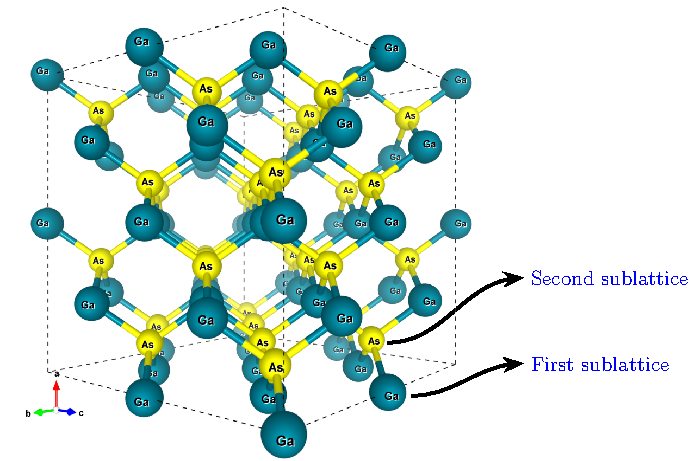
\includegraphics[width=\linewidth]{../figures/chapter-1/bulk-1/build/bulk-1}
	\caption{
		 GaAs crystal lattice, where the each sublattice correspond of each atom species Ga and As. }
	\label{fig:subsubsection-1.1.1-bulk-1}
\end{figure}


As before mentioned several times, it's very complex to compute the Schrödinger equation in the solids. The most ``exact'' compute is employed by DFT theory,  these calculations commonly are called atomistic even some  semiempirical models can consider as atomistic, but the semiemprical models are good approximations in comparison with the DFT theory. So, which is the reason to call ``exact'' solutions to the DFT results? The answer leads us to great discussion and  it's not intended to get into controversy,  but in general the DFT calculations have the capacity to calculate in terms of electrons interaction and the empirical methods are based in potential choice.\\
 
We will, don't into details about band calculations theories and models, but we will make a general reference to the importance in this work. The models more performed in semiconductor heterostructures as GaAs/AlGaAs are semiempirical, this is because DFT theory and their derived models are very limited to carried out in large structures, their electron interaction nature need high computational perform. So that in comparison with empirical models where the main role is the potential of semiconductor structures, this reduces computational reduce. So, the most models used in semiconductor band calculations are empirical models, these models are distinguished by low computational requires for this reason are considered like approximations. The importance to discuss these concepts will take relevance when we discuss the physics model proposed in this work. 

\begin{figure}[h!]\label{fig:subsubsection-1.1.1-GaAsbands-1}
	\centering
	\begin{subfigure}{\textwidth}
	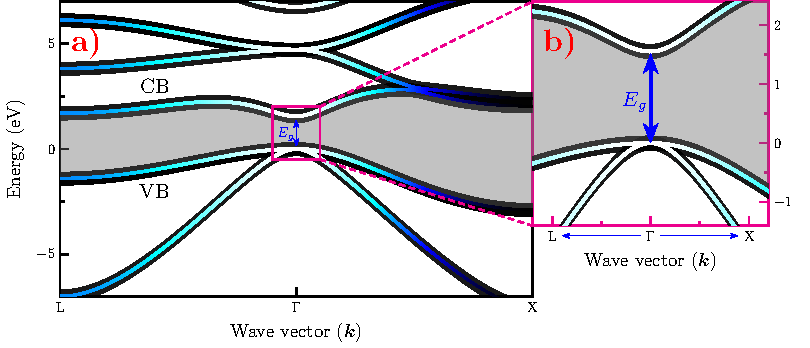
\includegraphics[width=\linewidth]{../figures/chapter-1/bands/build/bands01}
	\phantomsubcaption\label{subfig:subsubsection-1.1.1-GaAsbands-1-a)}
	\phantomsubcaption\label{subfig:subsubsection-1.1.1-GaAsbands-1-b)}
\end{subfigure}
	\caption{Band structure of GaAs, \subref{subfig:subsubsection-1.1.1-GaAsbands-1-a)} hows the zoom around of $\Gamma$  to denote the direct band gap and the electrons energy  needed to jump from valence to conduction band. \subref{subfig:subsubsection-1.1.1-GaAsbands-1-b)} denotes the two directions to dispersion of the bands corresponds to Brillouin zone: $\Gamma\to\mathrm{X}$ and  $\Gamma\to\mathrm{L}$.\cite{fox2002optical}}
\end{figure}

The \Cref{fig:subsubsection-1.1.1-GaAsbands-1} shows the results of calculations of TB model as discus it in \cite{vogl1983asemiempirical} and the code was impmemented by R. Muller \cite{rpmuller2017}. The model purposes by Vogl et al.  take into account small number of localized pseudo-orbitals and based the empirical parameters to substituted on TB Hamiltonian. 
The importance to get bandstructure it's based  importance to study optical properties of solid structures, if it doesn't exist  band electrons it's like look a place without map, so, the band structure  far from being  a complex tool it's the key to get the information to investigate the optical properties. 

As shown in \Cref{subfig:subsubsection-1.1.1-GaAsbands-1-a)} the GaAs bandstructure shows that it's a direct semiconductor as a previously mentioned, this gives way to get electron transitions from VB to CB and the energy to success this it. In \Cref{subfig:subsubsection-1.1.1-GaAsbands-1-b)} it's plotted, the band dispertion around $\Gamma$ point, it's the most symmetry point.  It is well-known that the band dispersion increasing $\boldsymbol{k}$ along two different directions of the Brillouin zone, from $\boldsymbol{k}=(0,0,0)$ to X point $\boldsymbol{k}=(2\pi a_{L})(1,0,0)$ and L point $\boldsymbol{k}=(2\pi a_{L})(1,1,1)$.  So, these figures, are the typical representation of direct gap to III-V semiconductors around of  $\boldsymbol{k}=0$, then, is obviously that the shape of dispersion is parabolic. For the GaAs bandstructure calculations shown in \Cref{fig:subsubsection-1.1.1-GaAsbands-1} doesn't take into account the contribution of spin\footnote{This spin contribution as called as split-off (so) hole band.}, therefore it's focus on three bands dispersion correspond to a single $s$-like conduction band and two $p$-like valence bands.  Is important to say that the characteristic curvature $E\!\!-\!\!\boldsymbol{k}$ of dispersion bands corresponds to an electron ($e$) in case of positive curvature while the negative curvature correspond to holes states; heavy ($hh$) and light hole ($lh$) bands, so, this denotes that the transitions, are of dipole nature\cite{fox2002optical,cardona2005fundamentals}. 
\begin{figure}[h!]
	\centering
		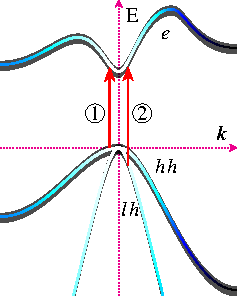
\includegraphics[width=0.5\linewidth]{../figures/chapter-1/bands/build/bands02}
	\caption{Two typical transitions for GaAs near $\boldsymbol{k}=0$. The first one correspond to the heavy-hole and second one to the light-hole. }
	\label{fig:subsubsection-1.1.1-GaAsbands-2}
\end{figure}
All the above disputed is significant to refers of one of the most indispensable quantum mechanisms in solids, this is absorption. The electron absorption, specifically interband absorption, give way to a fundamental physical process that involves the principle of many basic studies of semiconductors, applications, and the importance to understand the electron behavior in a semiconductor structures disputed in this work. Then the \Cref{fig:subsubsection-1.1.1-GaAsbands-2} schematizes the two typical transitions in GaAs bulk, this transitions are near to k=0, so that is called interband absorption. Is important to remark that the interband transitions are observed in all solids, but the mechanisms are different dependently of their bandstructure, for what,  being repetitive when mentioning that the bandstructure is the key to study solids. 

In case of GaAs the interband tranisitions are called as direct transitions, this is because their bandstructure proofs GaAs is a direct Gap semiconductor.  This process is determined by quantum mechanical rate $W_{i\to f}$ for exciting and electron in a initial quantum state $\psi_{i}$ to final state $\psi_{f}$ by absorption of a photon of angular frequency $\omega$\cite{fox2002optical}. As is very know, this is given by Fermi's golden rule. Later this is disputed according to highlight the model and results obtained. It has been mentioned that the direct transitions are of dipole nature, as before mentioned the CB is type $s$-like while the VB is $p$-like, then it've electric-dipole allowed transitions $p\to s$. The excitation of electron in CB carries to leave an initial state unoccupied, this is called as a hole creation, then the electron in the final state and the hole is considered as \textbf{electron-hole pair}. The next part subject this theme with major focus.


\subsection{Excitons}
\label{subsec:chapter-1-excitons}
\vspace{-10mm}
The importance to study bandstrcuture of semiconductors is very clear so far, so that could be said that absorption process is the source of optical properties of solids. It's due to this that the importance to study of semiconductors in the optoelectronics applications. But, this process give rise to formation of one of the most important excitations in the crystal structures. The photon absorption process carries to an electron is excited from CB to VB, this  generates an empty location in VB which has positive charge. This positive empty location called as hole, therefore the electron and hole have opposite charge then it's  to be expected that they are attracted, so, this creates a bound state called an exciton\cite{leonard2017exciton}. 

From \Cref{fig:subsubsection-1.1.1-GaAsbands-2} and \Cref{fig:subsubsection-1.1.1-x-1}  is clearly that excitons are commonly presented in direct band gap semiconductors as GaAs, this was denoted by absorption experiments,  after mentioned in \Cref{subsec:chapter-3-pl} this is the cause in photoluminiscence mechanism.

\begin{figure}[b]
	\centering
	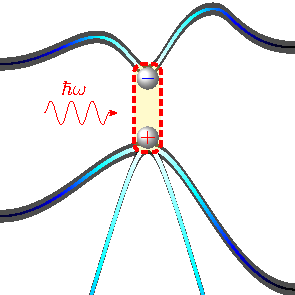
\includegraphics[width=0.5\linewidth]{../figures/chapter-1/exciton-1/build/x-1}
	\caption{Qualitative scheme of exciton creation in GaAs as direct gap.}
	\label{fig:subsubsection-1.1.1-x-1}
\end{figure}

\section{Semiconductor Low-Dimensional Structures}
\label{sec:chapter-1-low-dimensional-structures}
\vspace{-10mm} 
The previous section engaged to explain the principles of semiconductors, this is the bandstructure, the importance of these is practically the fingerprint of all semiconductor, without bandstructure  the understanding of these would be improbable. The first approximations were based in  GaAs bulk, their cubic symmetry practically defines their nature and consequently the physical effects as excitons existence.  But, what happens  if joined several semiconductors with same symmetry and structural parameters? The bulk properties and physical properties are the same?. 
The answers they are well-known, when two materials with relatively same structural parameters, as lattice constant can create a heterojunction, the union of several heterojunction make up a heterostructure.\footnote{The samples studied in this work are heterostructures, for this reason, and by nomenclature it's we refer to that way.}\\*
\begin{figure}[h]
	\centering
	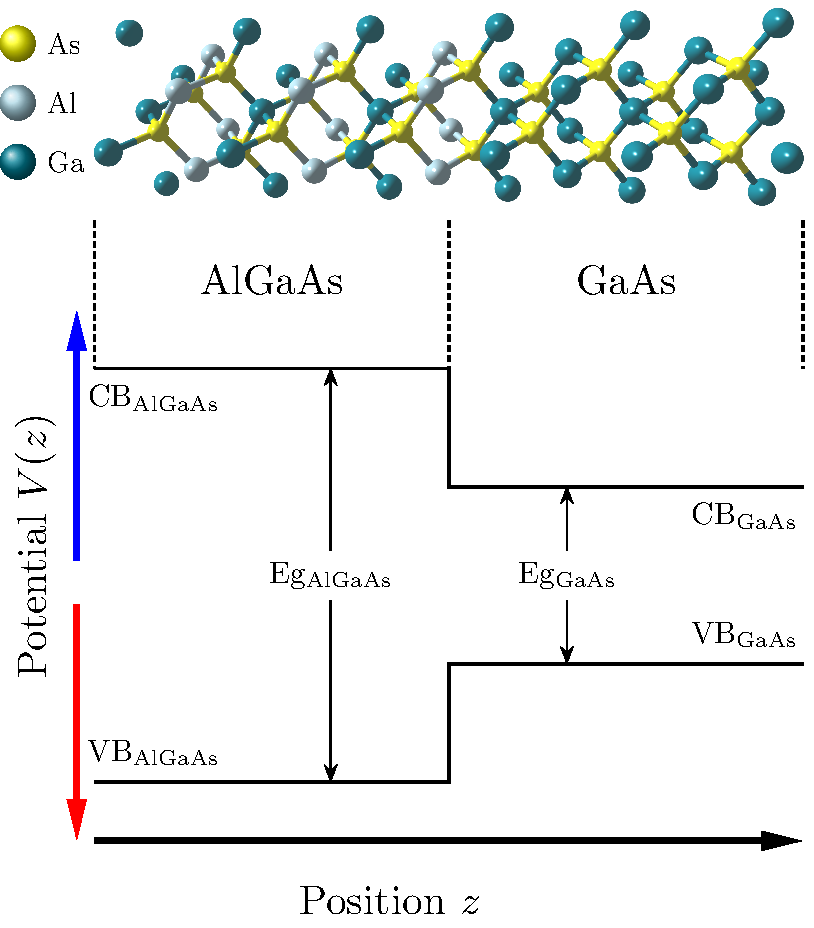
\includegraphics[width=0.65\textwidth]{../figures/chapter-1/heterostructures/out/hs-01}
	\caption{General scheme of GaAs/\algaas heterostructure, at top show the scheme of atomic arranged of this heterjunction, the dashed lines are the matched between two dissimilar materials. In bottom shows the band-edge profile.}
	\label{fig:subsection-1.2-heterostructure}
\end{figure}
The \Cref{fig:subsection-1.2-heterostructure} is a general scheme of a heterostructure, in this case is presents three species of atoms Al, As, Ga. These atoms can   locate in columns III-V of the periodic table, hence its name of III-V semiconductors. The principal characteristic of these atoms is that it can create matched structures as GaAs, AlAs and ternary alloys as \algaas with specific Al concentration. The matched semiconductors produce a material with new properties based principally in the difference of bandgap which involves the alloys. \\* 
As can see in \Cref{fig:subsection-1.2-heterostructure} it's consisting a GaAs/\algaas heterostructure, these interface is well-matched due to the lattice parameters is relatively equals, therefore and thanks to powerful growth technics as MBE it's possible to get high-quality quantum structures. 

Also, the heterostructure composed by two semiconductors with different band gaps generate a discontinuity in either the conduction or the valence band can be represented by a constant potential term\cite{harrison2016quantum}.  The theory to treatment the electron behavior in these structures, is relatively simple if we consider the above. 
Although, in this chapter doesn't have intention to explore the theory of electron behavior in that, worth noting that  it get one-dimensional potential $V(z)$ to both bands, so the Schr\"odinger equation can solve simple. 



\subsection{Quantum wells}
\label{subsection:chapter-1-quantum-wells}
\vspace{-10mm} 
Doubtless the creation or growth of heterostructures increased the interest in the study of quantum structures, the interactions, and physical behavior of light-matter they would not have been possible without these.  The major relevance is due the quantum confinement, the junction of semiconductors results in an interest quantum structures with specific dimensions. From 3D bulk the dimensions reduce to 2D,1D and 0D dimensional structures. Therefore each of that has interest properties and their correspond applications. The \Cref{fig:subsection-1.2-heterostructures} schematics the low dimensional heterostructures from 3D bulk, the first low dimensional from 3D to 2D  is the Quantum Wells, then from 2D to 1D it have the Quantum Wires finally with 0D have the Quantum Dots.
\begin{figure}
	\centering
	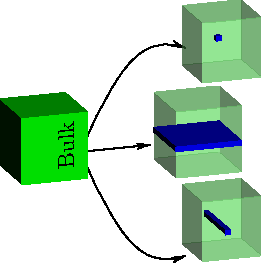
\includegraphics[width=0.6\textwidth]{../figures/chapter-1/heterostructures/out/lds-00}
	\caption{Heterostructures from bulk (3D), to Quantum Wells (2D), Quantum Wires (1D) and Quantum Dots (0D).  }
	\label{fig:subsection-1.2-heterostructures}
\end{figure}
The quantum confinement so is the principal reason to study that structures, the electron behavior which exhibits in it  should  can to help  understand  a great variety of quantum mechanical phenomena as electron interaction on a crystal. 
Suppose a heterostructure composed with a two semiconductor alloys as sandwich, this 2D quantum structure is called a Single Quantum Well (SQW). \\*
This dissimilar semiconductors in terms of their potential energy ($V(z)$) can be schematized as \Cref{fig:subsection-1.2-single-quantum-well-scheme}. The Gap difference of \algaas and GaAs is due to $x$ Al concentration in \algaas therefore it obtains a one dimensional potential profile, with that can confinement electrons in a 2D plane along $z$ direction. 
All of these carries to quantum mechanics formalism, the electron behavior should be obeyed these rules. If we have an electron closed in two potential barriers  an $L$ distance, the wave which describe it will be spatially confined.
So if we confined many electrons in these potential,  we have two important physical aspects: the first one is knowing as Pauli's exclusion principle, which as of its Fermion nature prevents carriers with the same spin occupying the same region in of space\cite{harrison2016quantum,pauli1925zusammenhang}, the second one and one of the most relevant in the birth of the quantum mechanics; the Heisenberg's uncertainty principle. 
That last, it can say  that is the consequence of quantum confinement due to the space reduction of the electrons is expected that momentum increases by an amount of the order $\hbar/L$. Therefore, the energy of that confined particles increases, and it's referred to as confinement energy\cite{cardona2005fundamentals}. \\*
\begin{figure}
	\centering
	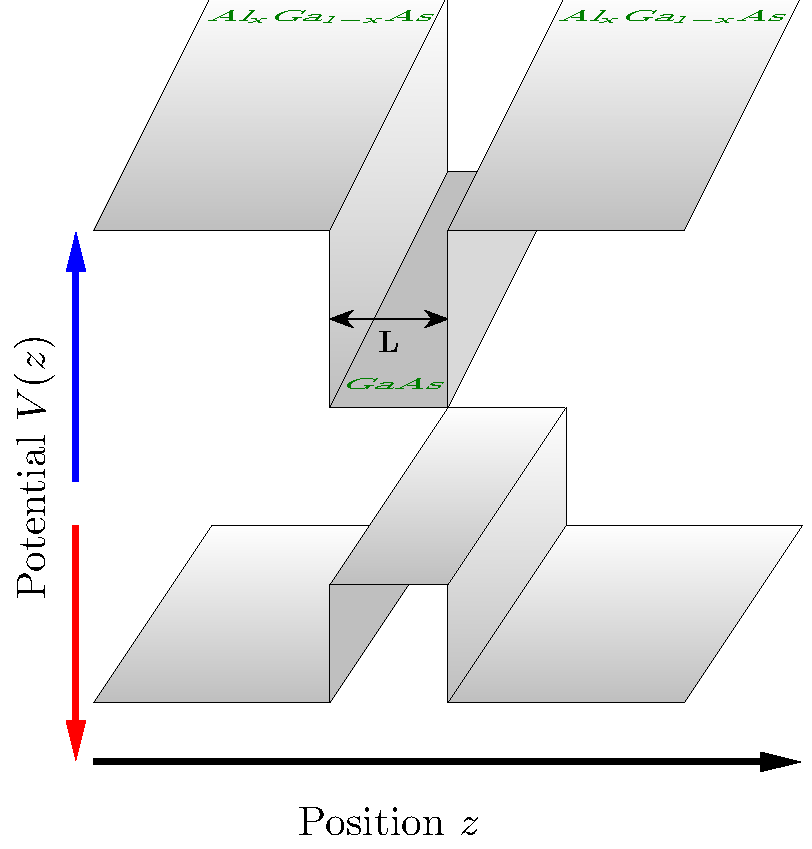
\includegraphics[width=0.65\textwidth]{../figures/chapter-1/heterostructures/out/qw1}
	\caption{GaAs/\algaas Single Quantum Well }
	\label{fig:subsection-1.2-single-quantum-well-scheme}
\end{figure}
Then the quantum confinement is our started point to understand the optical properties in QWs. As is referred in the figure, the uni-dimensional potential profile can well describe by top conduction- and bottom valence-bands, the band offset in these two of correspond gap energy between that, while Al concentration increases their bandgap and the band offset ($\mathrm{Q_{c}}$ to CB and $\mathrm{Q_{v}}$ to VB) also to.   

It's so clearly  that the QWs have the potential to presents amazing quantum properties, even if all of these are very important we focus on the optical properties, basically our interest is the light-matter interaction through its result mechanisms.  
 
\subsection{Preliminary approach of Quantum Confinement effect in QWs}
\label{subsection:chapter-1-preliminary-approach-of-quantum-confinment-effect-in-qws}
\vspace{-10mm} 
As the title describes, here it will try to explain as the first  approach the quantum confinement effect in QWs. If  it starts with the  scoop, which it can be reduced the electrons space, then this mean that in reciprocal space it has two components $k_{x}$ and $k_{y}$. Then say in crystal symmetry properties to the case of GaAs/\algaas QWs it's $\Gamma$ the central point, as long as $x < 0.4$\footnote{It will be explained in the next section, although it's due to the Gap go from direct to indirect, shortly the symmetry $\Gamma\to X$.} the bandstructure depends on confinement energ, so say which the bandstructure depends on confinement energy.  
In this case, the electronic properties in comparison with a bulk semiconductor properties can solve trough particle-in-a-box as textbook problem as first approach. Nevertheless, even if usually can solver without much mathematical formalism is very essential that it dedicates a chapter with their solution, this is because will employ a physical formalism exclusively to QWs structures. In general way, as it before mentioned the Schrödinger equation solution is the fundamental pillar to understand, where it's taken into account which  in a crystal the periodic potential is the key. Here are important remarks before to continue, when it has a heterostructure starting with the bulk model it's clearly that the system doesn't same, the Quantum Mechanics which is behind take into account the symmetry properties, then it can be developed a Hamiltonian  to understand that system.  In the next chapter will be explained details and the formalism both physical and mathematical to solve and discus it's. The model which give the tools to get the solutions is called as Effective Mass Approximation, thus their correspond Schrödinger equation is\cite{harrison2016quantum,chuang1995physics,singh2003electronic,bastard1990wave,fox2002optical,davies1998physics}: 
\begin{equation}\label{eq:chapter-1-ema-schroedinger}
	-\dfrac{\hbar^{2}}{2m^{*}}\dfrac{\partial^{2}}{\partial {z}^{2}}\psi(z)+V(z)\psi(z)=E\psi(z),
\end{equation}

where the $m^{*}$ is the effective mass in each material, and $V(z)$ is the potential profile got by heterostructure materials properties. Therefore, that differential equation can solve as in textbooks explained\cite{de2014introduccion,griffiths2018introduction,sakurai1995modern,cohen2019quantum,chuang1995physics,harrison2016quantum,fox2002optical,bastard1990wave}. The idea is thinking as a one particle in a finite potential well, where is well important established the boundary conditions and solve the Schrödinger equation in each part of single QW, this means that need to create a potential function. Then it's can obtain the Eigenfunctions and their correspond Eigenenergies.

\begin{figure}
	\begin{subfigure}{\textwidth}
		\centering
		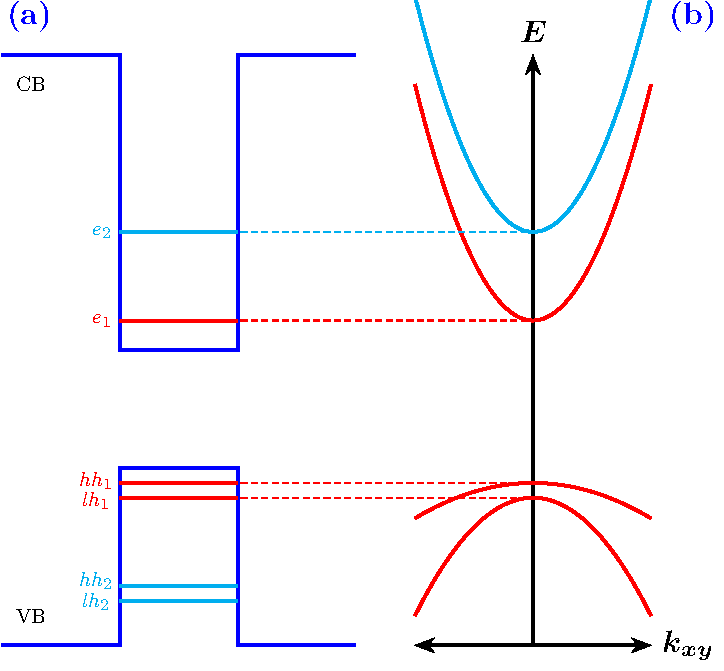
\includegraphics[width=0.65\textwidth]{../figures/chapter-1/heterostructures/out/qw2}
		\phantomsubcaption\label{subfig:subsection-1.2-single-quantum-well-scheme2-a)}
		\phantomsubcaption\label{subfig:subsection-1.2-single-quantum-well-scheme2-b)}
	\end{subfigure}
	\caption{General scheme of typical Schrödinger's equation solutions to one-dimensional potential as \subref{subfig:subsection-1.2-single-quantum-well-scheme2-a)} where the Eigenenergies of both electron and holes are denoted with same color depending on  $n$ value.\subref{subfig:subsection-1.2-single-quantum-well-scheme2-b)} It's plot, of the subbands in  the same case of  \subref{subfig:subsection-1.2-single-quantum-well-scheme2-a)} to both particles.  }
	\label{fig:subsection-1.2-single-quantum-well-scheme2}
\end{figure}

The principal idea doesn't is reproducing something which is very well known, the objective of this part is established the scoop of the next chapter. Therefore,  before to continue, we will finish with to explain the dispersion in-plane of single QW. As in the QW the one-dimensional potential set up the 1D confinement, is important doesn't confuse which the QW is a 2D structure, but their confinement is along of $z$ direction  this mean 1D. Then, the particle can motion in the $x-y$ plane. By this reason, even if consider 3D Schrödinger equation and  the above is considered it obtain \Cref{eq:chapter-1-ema-schroedinger}
therefore, the solutions in the one-dimensional potential produce discrete states of energy $E_{z}=E_{n}$\cite{harrison2016quantum}, where $n$ is the energy level it which produce  subbands as shows in \Cref{fig:subsection-1.2-single-quantum-well-scheme2}. In contrast, before it called as ``energy bands'' in the bulk case, now due to the quantum confinement gets subbands to both conduction- and valence bands.

These subbands are the result of the sum of $E_{z}$ and $E_{x,y}$, which are the 1D confinement energy and the in-plane momentum $k_{x,y}$ then\cite{harrison2016quantum}:
\begin{equation}\label{eqn:chapter-1-total-enery-ema-aprox}		
	E = E_{n} + \dfrac{\hbar^{2}|\boldsymbol{k}_{x,y}|^{2}}{2m^{*}}.
\end{equation}  
From equation the effective mass  $m^*$ depends on particle, i.e the effective mass to electrons in CB and the holes in VB. So, the most relevant in the solutions is the energy $E_{n}$ (\Cref{subfig:subsection-1.2-single-quantum-well-scheme2-a)})  is discrete, this is the quantum confinement in the low-dimensional heterostructures. 


\section{Summary}
\vspace{-10mm} 
In this chapter, was exposed the generalities of semiconductor band structure and low-dimensional heterostructures, highlighting or taking in major GaAs/\algaas that's the semiconductors of major importance in this work. 
The band structure interpretation  usually be so hard, and their calculations even more, but the impact and relevance in optical properties of semiconductors starts from that interpretation, from here arises the mathematical arsenal to right physical interpretation. Another significant concept which was treatment as first approach is the effective mass concept, even if, when solved, the bulk Hamiltonian it considers the mass as constant parameter or depending on semiconductor material, contrary  in low-dimensional structures have an important role.  \\*

In generally, the band structure of semiconductors is the key to understand quantum properties of solids, in this work the  relevant is the light-matter. Remember that light-mater interaction in solids can be studied by process resulting in it, as absorption, reflection, transmission, diffraction, scattering, and others\cite{rivera2020light}.  Although, the light-matter interactions are fundamentally  quantum electrodynamical, also, can be studied in quantum way through before mentioned process. Firstly, is the photon absorption process can help to understand or calculate the fundamental parameter in semiconductors as is bandgap energy. 
This parameter is the started point in the study of semiconductors, this is the start point in the map called bandstructure, if it ignores the gap value in the semiconductor to study it couldn't possibly get the principal optical properties of that. \\*
Then, the bandstructure of semiconductors is the map to understand them, without these routes or fundamental parameters couldn't have quantum devices. 
 
